\documentclass[a4paper,12pt]{article}
%\documentclass[fleqn]{article}

% ---パッケージ---
\usepackage{amsmath,amssymb}    %数式用
\usepackage{tcolorbox}   %囲み枠用(tcolorboxに変更)
\usepackage{geometry}   %余白調節
\usepackage{tikz}  % ← 図を描くためのTikZパッケージ
\geometry{margin=25mm}  %余白を少し狭く
\usetikzlibrary{decorations.pathmorphing,patterns,positioning,arrows.meta} % バネ・壁の模様
\tikzset{
  block/.style = {draw, rectangle, minimum height=2em, minimum width=3em},
  sum/.style = {draw, circle, inner sep=0pt, minimum size=5mm},
  input/.style = {coordinate},
  output/.style = {coordinate}
}
\usetikzlibrary{calc}

% --- 日本語用パッケージ ---
\usepackage{luatexja}         % 日本語表示に必要
\usepackage{luatexja-fontspec} % フォント指定用

% --- フォント指定(Overleaf標準フォント)---
\setmainjfont{IPAexMincho}  % 明朝体
%\setmainjfont{IPAexGothic}  % ゴシック体にしたい場合

% --- tcolorbox の設定 ---
\tcbset{
  colframe=black,
  colback=white,         % 本文の背景(白)
  boxrule=0.8pt,
  arc=3pt,
  outer arc=3pt,
  boxsep=4pt,
  coltitle=black,
  colbacktitle=gray!20,  % タイトルの背景(グレー)
  fonttitle=\normalsize
}

\begin{document}

\begin{tcolorbox}[title={[1] ブロック線図を簡単にせよ. 
\begin{center}
\begin{tikzpicture}[auto, node distance=0.4cm and 0.6cm, >=Latex]
  % --- 主系列ノード ---
  \node at (0,0) (input) {};
  \node[circle, draw, inner sep=1.5pt, right=of input] (sum1) {};         % 合流点1
  \node[block, right=of sum1] (G1) {$G_1$};
  \node[circle, fill=black, inner sep=1.5pt, right=of G1] (branch1) {};   % 分岐点1
  \node[block, right=of branch1] (G2) {$G_2$};
  \node[circle, fill=black, inner sep=1.5pt, right=of G2] (branch2) {};   % 分岐点2
  \node[block, right=of branch2] (G3) {$G_3$};
  \node[circle, draw, inner sep=1.5pt, right=of G3] (sum2) {};           % 合流点2
  \node[right=of sum2] (output) {};
  
  % --- 上部ノード(分岐2の上にG4) ---
  \node[block, above=0.6cm of branch2] (G4) {$G_4$};
  
  % --- 下部ノード(G1の下にH1、さらにその下にH2) ---
  \node[block, below=0.6cm of G1] (H1) {$H_1$};
  \node[block, below=0.6cm of H1] (H2) {$H_2$};

  % === 主系列経路 ===
  \draw[->] (input) -- (sum1);
  \draw[->] (sum1) -- (G1);
  \draw[->] (G1) -- (branch1);
  \draw[->] (branch1) -- (G2);
  \draw[->] (G2) -- (branch2);
  \draw[->] (branch2) -- (G3);
  \draw[->] (G3) -- (sum2);
  \draw[->] (sum2) -- (output);
  
  % === 追加経路 ===
  % 分岐1 → G4 → 合流2(カクカク経路)
  \draw[->] (branch1) |- (G4) -| (sum2);

  % 分岐1 → H1 → 合流1(カクカク経路)
  \draw[->] (branch1) |- (H1) -| (sum1);

  % 分岐2 → H2 → 合流1(カクカク経路)
  \draw[->] (branch2) |- (H2) -| (sum1);

  % --- 加算記号配置 ---
  \node at ($(sum1)+(-0.3,0.3)$) {\small $+$};
  \node at ($(sum1)+(0.3,-0.3)$) {\small $-$};
  \node at ($(sum2)+(-0.3,0.3)$) {\small $+$};
  \node at ($(sum2)+(-0.3,-0.3)$) {\small $+$};

  % --- ラベル ---
  \node at ($(sum1)+(-1.0,0.3)$) {\small $R(s)$};
  \node at ($(sum2)+(1.0,0.3)$) {\small $C(s)$};

\end{tikzpicture}
\end{center}

\vspace{2mm}
}]

\begin{center}

\begin{tikzpicture}[auto, node distance=0.4cm and 0.6cm, >=Latex]
  % --- 主系列ノード(G2とbranch2を交換) ---
  \node at (0,0) (input) {};
  \node[circle, draw, inner sep=1.5pt, right=of input] (sum1) {};         
  \node[block, right=of sum1] (G1) {$G_1$};
  \node[circle, fill=black, inner sep=1.5pt, right=of G1] (branch1) {};   
  \node[circle, fill=black, inner sep=1.5pt, right=1.2cm of branch1] (branch2) {}; % ← G2と交換された分岐点
  \node[block, right=of branch2] (G2_main) {$G_2$};                         % ← G2が後ろに
  \node[block, right=of G2_main] (G3) {$G_3$};
  \node[circle, draw, inner sep=1.5pt, right=of G3] (sum2) {};             
  \node[right=of sum2] (output) {};

  % --- 上部ノード(branch2の上にG4) ---
  \node[block, above=0.6cm of branch2] (G4) {$G_4$};

  % --- 下部ノード(G1の下にH1、G2→H2構成) ---
  \node[block, below=0.6cm of G1] (H1) {$H_1$};
  \node[block, below=0.6cm of H1] (H2) {$H_2$};
  \node[block, right=0.4cm of H2] (G2_fb) {$G_2$};  % ← G₂(H₂ルート用)
  

  % === 主系列経路 ===
  \draw[->] (input) -- (sum1);
  \draw[->] (sum1) -- (G1);
  \draw[->] (G1) -- (branch1);
  \draw[->] (branch1) -- (branch2);           % ← 分岐点2を前に
  \draw[->] (branch2) -- (G2_main);
  \draw[->] (G2_main) -- (G3);
  \draw[->] (G3) -- (sum2);
  \draw[->] (sum2) -- (output);

  % === 追加経路 ===
  \draw[->] (branch1) |- (H1) -| (sum1);
  \draw[->] (branch1) |- (G4) -| (sum2);
  \draw[->] (branch2) |- (G2_fb) -- (H2) -| (sum1);  % ← 正しく G₂ → H₂ → 合流1

  % --- 加算記号配置 ---
  \node at ($(sum1)+(-0.3,0.3)$) {\small $+$};
  \node at ($(sum1)+(0.3,-0.3)$) {\small $-$};
  \node at ($(sum2)+(-0.3,0.3)$) {\small $+$};
  \node at ($(sum2)+(-0.3,-0.3)$) {\small $+$};

  % --- ラベル ---
  \node at ($(sum1)+(-1.0,0.3)$) {\small $R(s)$};
  \node at ($(sum2)+(1.0,0.3)$) {\small $C(s)$};

\end{tikzpicture}


\vspace{2mm}
    
\begin{tikzpicture}
    \node {\Huge$\Downarrow$};
    \end{tikzpicture}
\vspace{2mm}


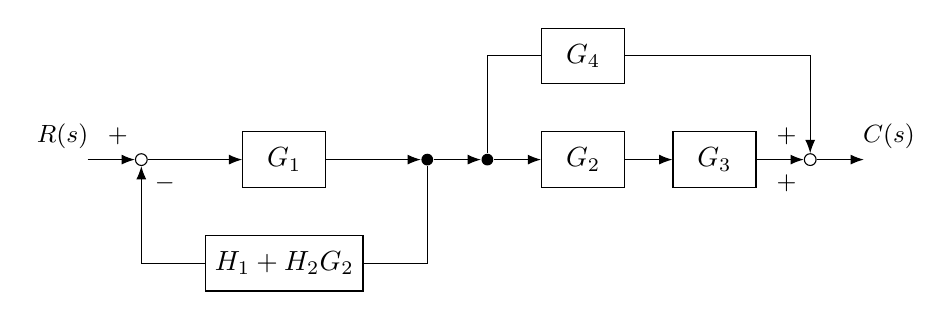
\begin{tikzpicture}[auto, node distance=0.4cm and 0.6cm, >=Latex]
  % --- 主系列ノード ---
  \node at (0,0) (input) {};
  \node[circle, draw, inner sep=1.5pt, right=of input] (sum1) {};         
  \node[block, right=1.2cm of sum1] (G1) {$G_1$};
  \node[circle, fill=black, inner sep=1.5pt, right=1.2cm of G1] (branch1) {};   
  \node[circle, fill=black, inner sep=1.5pt, right=of branch1] (branch3) {}; % ← 旧branch2削除済
  \node[block, right=of branch3] (G2_main) {$G_2$};
  \node[block, right=of G2_main] (G3) {$G_3$};
  \node[circle, draw, inner sep=1.5pt, right=of G3] (sum2) {};             
  \node[right=of sum2] (output) {};

  % --- 上部ノード(G2_mainの上にG4) ---
  \node[block, above=0.6cm of G2_main] (G4) {$G_4$};

  % --- 合成フィードバックノード(G1の真下) ---
  \node[block, below=0.6cm of G1] (Hfb) {$H_1 + H_2 G_2$};

  % === 主系列経路 ===
  \draw[->] (input) -- (sum1);
  \draw[->] (sum1) -- (G1);
  \draw[->] (G1) -- (branch1);
  \draw[->] (branch1) -- (branch3);
  \draw[->] (branch3) -- (G2_main);
  \draw[->] (G2_main) -- (G3);
  \draw[->] (G3) -- (sum2);
  \draw[->] (sum2) -- (output);

  % === 追加経路 ===
  \draw[->] (branch3) |- (G4) -| (sum2);           % 分岐3 → G4 → 合流点2
  \draw[->] (branch1) |- (Hfb) -| (sum1);          % 合成フィードバック → 合流点1

  % --- 加算記号配置 ---
  \node at ($(sum1)+(-0.3,0.3)$) {\small $+$};
  \node at ($(sum1)+(0.3,-0.3)$) {\small $-$};
  \node at ($(sum2)+(-0.3,0.3)$) {\small $+$};
  \node at ($(sum2)+(-0.3,-0.3)$) {\small $+$};

  % --- ラベル ---
  \node at ($(sum1)+(-1.0,0.3)$) {\small $R(s)$};
  \node at ($(sum2)+(1.0,0.3)$) {\small $C(s)$};

\end{tikzpicture}


\vspace{2mm}
    
\begin{tikzpicture}
    \node {\Huge$\Downarrow$};
    \end{tikzpicture}
\vspace{2mm}


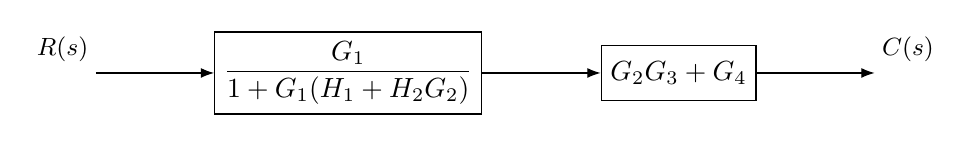
\begin{tikzpicture}[auto, node distance=1.0cm and 1.5cm, >=Latex]
  % --- 入出力とブロック ---
  \node at (0,0) (input) {};
  \node[block, right=of input] (Gleft) {$\dfrac{G_1}{1 + G_1 (H_1 + H_2 G_2)}$};
  \node[block, right=of Gleft] (Gright) {$G_2 G_3 + G_4$};
  \node[right=of Gright] (output) {};

  % --- 矢印 ---
  \draw[->] (input) -- (Gleft);
  \draw[->] (Gleft) -- (Gright);
  \draw[->] (Gright) -- (output);

  % --- ラベル ---
  \node at ($(input)+(-0.3,0.3)$) {\small $R(s)$};
  \node at ($(output)+(0.3,0.3)$) {\small $C(s)$};
\end{tikzpicture}


\vspace{2mm}
    
\begin{tikzpicture}
    \node {\Huge$\Downarrow$};
    \end{tikzpicture}
\vspace{2mm}


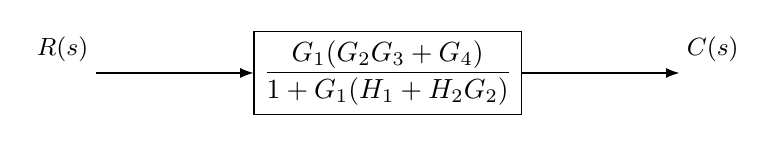
\begin{tikzpicture}[auto, node distance=1.2cm and 2.0cm, >=Latex]
  % --- 入出力とブロック ---
  \node at (0,0) (input) {};
  \node[block, right=of input] (Gtotal) 
    {$\dfrac{G_1 (G_2 G_3 + G_4)}{1 + G_1 (H_1 + H_2 G_2)}$};
  \node[right=of Gtotal] (output) {};

  % --- 矢印 ---
  \draw[->] (input) -- (Gtotal);
  \draw[->] (Gtotal) -- (output);

  % --- ラベル ---
  \node at ($(input)+(-0.3,0.3)$) {\small $R(s)$};
  \node at ($(output)+(0.3,0.3)$) {\small $C(s)$};
\end{tikzpicture}

\end{center}

\end{tcolorbox}

\begin{tcolorbox}[title={[2] ブロック線図を簡単にせよ. 
\begin{center}
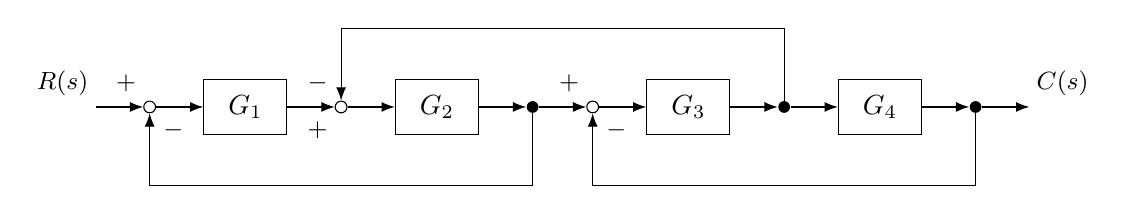
\begin{tikzpicture}[auto, node distance=0.4cm and 0.6cm, >=Latex]

  % --- 主系列ノード配置 ---
  \node at (0,0) (input) {};
  \node[circle, draw, inner sep=1.5pt, right=of input] (sum1) {};          % 合流1
  \node[block, right=of sum1] (G1) {$G_1$};
  \node[circle, draw, inner sep=1.5pt, right=of G1] (sum2) {};             % 合流2
  \node[block, right=of sum2] (G2) {$G_2$};
  \node[circle, fill=black, inner sep=1.5pt, right=of G2] (branch1) {};    % 分岐1
  \node[circle, draw, inner sep=1.5pt, right=of branch1] (sum3) {};        % 合流3
  \node[block, right=of sum3] (G3) {$G_3$};
  \node[circle, fill=black, inner sep=1.5pt, right=of G3] (branch2) {};    % 分岐2
  \node[block, right=of branch2] (G4) {$G_4$};
  \node[circle, fill=black, inner sep=1.5pt, right=of G4] (branch3) {};    % 分岐3
  \node[right=of branch3] (output) {};

  % --- 経由ポイント(カクカク折れ線用) ---
  \coordinate (pivot1) at ($(branch1)+(0,-1.0)$);  % branch1 → sum1
  \coordinate (pivot2) at ($(branch2)+(0,1.0)$);   % branch2 → sum2
  \coordinate (pivot3) at ($(branch3)+(0,-1.0)$);  % branch3 → sum3

  % === 主系列経路 ===
  \draw[->] (input) -- (sum1);
  \draw[->] (sum1) -- (G1);
  \draw[->] (G1) -- (sum2);
  \draw[->] (sum2) -- (G2);
  \draw[->] (G2) -- (branch1);
  \draw[->] (branch1) -- (sum3);
  \draw[->] (sum3) -- (G3);
  \draw[->] (G3) -- (branch2);
  \draw[->] (branch2) -- (G4);
  \draw[->] (G4) -- (branch3);
  \draw[->] (branch3) -- (output);

  % === 追加経路(折れ線) ===
  \draw[->] (branch1) -- (pivot1) -| (sum1);
  \draw[->] (branch2) -- (pivot2) -| (sum2);
  \draw[->] (branch3) -- (pivot3) -| (sum3);

  % --- 加算記号配置 ---
  \node at ($(sum1)+(-0.3,0.3)$) {\small $+$};
  \node at ($(sum1)+(0.3,-0.3)$) {\small $-$};

  \node at ($(sum2)+(-0.3,0.3)$) {\small $-$};
  \node at ($(sum2)+(-0.3,-0.3)$) {\small $+$};

  \node at ($(sum3)+(-0.3,0.3)$) {\small $+$};
  \node at ($(sum3)+(0.3,-0.3)$) {\small $-$};

  % --- 入出力ラベル ---
  \node at ($(input)+(-0.3,0.3)$) {\small $R(s)$};
  \node at ($(output)+(0.3,0.3)$) {\small $C(s)$};

\end{tikzpicture}
\end{center}

\vspace{2mm}
}]

\begin{center}

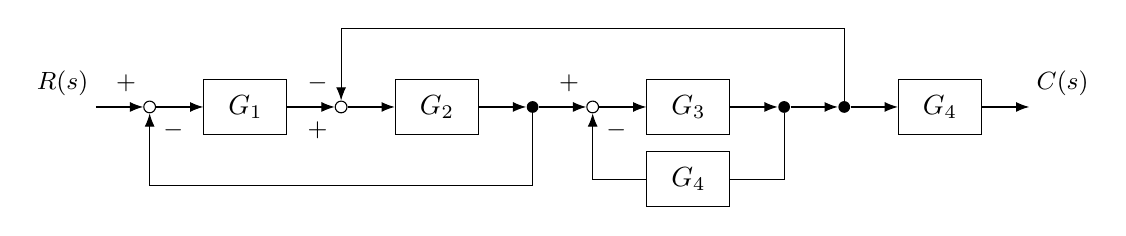
\begin{tikzpicture}[auto, node distance=0.4cm and 0.6cm, >=Latex]

  % --- 主系列ノード配置 ---
  \node at (0,0) (input) {};
  \node[circle, draw, inner sep=1.5pt, right=of input] (sum1) {};         
  \node[block, right=of sum1] (G1) {$G_1$};
  \node[circle, draw, inner sep=1.5pt, right=of G1] (sum2) {};            
  \node[block, right=of sum2] (G2) {$G_2$};
  \node[circle, fill=black, inner sep=1.5pt, right=of G2] (branch1) {};   
  \node[circle, draw, inner sep=1.5pt, right=of branch1] (sum3) {};       
  \node[block, right=of sum3] (G3) {$G_3$};
  \node[circle, fill=black, inner sep=1.5pt, right=of G3] (branch3) {};   % 分岐3:G3と分岐2の間
  \node[circle, fill=black, inner sep=1.5pt, right=of branch3] (branch2) {}; 
  \node[block, right=of branch2] (G4_main) {$G_4$};                       % 主系列上のG4
  \node[right=of G4_main] (output) {};

  % --- G4(追加ルート用) ---
  \node[block, below=0.2cm of G3] (G4_fb) {$G_4$}; % G3の下

  % --- 経由ポイント ---
  \coordinate (pivot1) at ($(branch1)+(0,-1.0)$);  % branch1 → sum1
  \coordinate (pivot2) at ($(branch2)+(0,1.0)$);   % branch2 → sum2

  % === 主系列経路 ===
  \draw[->] (input) -- (sum1);
  \draw[->] (sum1) -- (G1);
  \draw[->] (G1) -- (sum2);
  \draw[->] (sum2) -- (G2);
  \draw[->] (G2) -- (branch1);
  \draw[->] (branch1) -- (sum3);
  \draw[->] (sum3) -- (G3);
  \draw[->] (G3) -- (branch3);
  \draw[->] (branch3) -- (branch2);
  \draw[->] (branch2) -- (G4_main);
  \draw[->] (G4_main) -- (output);

  % === 追加経路 ===
  \draw[->] (branch1) -- (pivot1) -| (sum1);
  \draw[->] (branch2) -- (pivot2) -| (sum2);
  \draw[->] (branch3) |- (G4_fb) -| (sum3);  % ← G4経由の戻りルート

  % --- 加算記号配置 ---
  \node at ($(sum1)+(-0.3,0.3)$) {\small $+$};
  \node at ($(sum1)+(0.3,-0.3)$) {\small $-$};

  \node at ($(sum2)+(-0.3,0.3)$) {\small $-$};
  \node at ($(sum2)+(-0.3,-0.3)$) {\small $+$};

  \node at ($(sum3)+(-0.3,0.3)$) {\small $+$};
  \node at ($(sum3)+(0.3,-0.3)$) {\small $-$};

  % --- ラベル ---
  \node at ($(input)+(-0.3,0.3)$) {\small $R(s)$};
  \node at ($(output)+(0.3,0.3)$) {\small $C(s)$};

\end{tikzpicture}


\vspace{2mm}
    
\begin{tikzpicture}
    \node {\Huge$\Downarrow$};
    \end{tikzpicture}
\vspace{2mm}

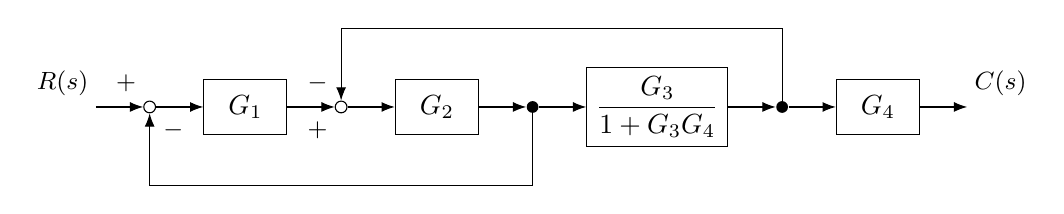
\begin{tikzpicture}[auto, node distance=0.4cm and 0.6cm, >=Latex]

  % --- 主系列ノード配置 ---
  \node at (0,0) (input) {};
  \node[circle, draw, inner sep=1.5pt, right=of input] (sum1) {};         
  \node[block, right=of sum1] (G1) {$G_1$};
  \node[circle, draw, inner sep=1.5pt, right=of G1] (sum2) {};            
  \node[block, right=of sum2] (G2) {$G_2$};
  \node[circle, fill=black, inner sep=1.5pt, right=of G2] (branch1) {};   
  \node[block, right=of branch1] (G3_fb) {$\dfrac{G_3}{1 + G_3 G_4}$};     % フィードバック済
  \node[circle, fill=black, inner sep=1.5pt, right=of G3_fb] (branch2) {}; 
  \node[block, right=of branch2] (G4_main) {$G_4$};
  \node[right=of G4_main] (output) {};

  % --- 経由ポイント ---
  \coordinate (pivot1) at ($(branch1)+(0,-1.0)$);  % branch1 → sum1
  \coordinate (pivot2) at ($(branch2)+(0,1.0)$);   % branch2 → sum2

  % === 主系列経路 ===
  \draw[->] (input) -- (sum1);
  \draw[->] (sum1) -- (G1);
  \draw[->] (G1) -- (sum2);
  \draw[->] (sum2) -- (G2);
  \draw[->] (G2) -- (branch1);
  \draw[->] (branch1) -- (G3_fb);
  \draw[->] (G3_fb) -- (branch2);
  \draw[->] (branch2) -- (G4_main);
  \draw[->] (G4_main) -- (output);

  % === 追加経路 ===
  \draw[->] (branch1) -- (pivot1) -| (sum1);
  \draw[->] (branch2) -- (pivot2) -| (sum2);

  % --- 加算記号配置 ---
  \node at ($(sum1)+(-0.3,0.3)$) {\small $+$};
  \node at ($(sum1)+(0.3,-0.3)$) {\small $-$};

  \node at ($(sum2)+(-0.3,0.3)$) {\small $-$};
  \node at ($(sum2)+(-0.3,-0.3)$) {\small $+$};

  % --- ラベル ---
  \node at ($(input)+(-0.3,0.3)$) {\small $R(s)$};
  \node at ($(output)+(0.3,0.3)$) {\small $C(s)$};

\end{tikzpicture}



\vspace{2mm}
    
\begin{tikzpicture}
    \node {\Huge$\Downarrow$};
    \end{tikzpicture}
\vspace{2mm}

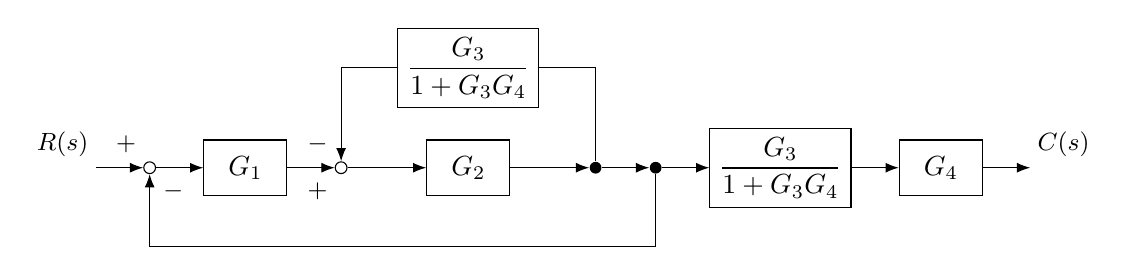
\begin{tikzpicture}[auto, node distance=0.4cm and 0.6cm, >=Latex]

  % --- 主系列ノード配置 ---
  \node at (0,0) (input) {};
  \node[circle, draw, inner sep=1.5pt, right=of input] (sum1) {};         
  \node[block, right=of sum1] (G1) {$G_1$};
  \node[circle, draw, inner sep=1.5pt, right=of G1] (sum2) {};            
  \node[block, right=1.0cm of sum2] (G2) {$G_2$};
  \node[circle, fill=black, inner sep=1.5pt, right=1.0cm of G2] (branch2) {};   % ← 分岐2
  \node[circle, fill=black, inner sep=1.5pt, right=of branch2] (branch1) {};   
  \node[block, right=of branch1] (G3_fb) {$\dfrac{G_3}{1 + G_3 G_4}$};     % フィードバック済
  \node[block, above=0.4cm of G2] (G3_fb_dup) {$\dfrac{G_3}{1 + G_3 G_4}$}; % 分岐2→sum2用
  \node[block, right=of G3_fb] (G4_main) {$G_4$};
  \node[right=of G4_main] (output) {};

  % --- 経由ポイント(1のみ残す) ---
  \coordinate (pivot1) at ($(branch1)+(0,-1.0)$);  % branch1 → sum1

  % === 主系列経路 ===
  \draw[->] (input) -- (sum1);
  \draw[->] (sum1) -- (G1);
  \draw[->] (G1) -- (sum2);
  \draw[->] (sum2) -- (G2);
  \draw[->] (G2) -- (branch2);
  \draw[->] (branch2) -- (branch1);
  \draw[->] (branch1) -- (G3_fb);
  \draw[->] (G3_fb) -- (G4_main);
  \draw[->] (G4_main) -- (output);

  % === 追加経路 ===
  \draw[->] (branch1) -- (pivot1) -| (sum1);
  \draw[->] (branch2) |- (G3_fb_dup) -| (sum2);   % ← pivot2 削除、直接 |- 接続

  % --- 加算記号配置 ---
  \node at ($(sum1)+(-0.3,0.3)$) {\small $+$};
  \node at ($(sum1)+(0.3,-0.3)$) {\small $-$};

  \node at ($(sum2)+(-0.3,0.3)$) {\small $-$};
  \node at ($(sum2)+(-0.3,-0.3)$) {\small $+$};

  % --- ラベル ---
  \node at ($(input)+(-0.3,0.3)$) {\small $R(s)$};
  \node at ($(output)+(0.3,0.3)$) {\small $C(s)$};

\end{tikzpicture}


\vspace{2mm}
    
\begin{tikzpicture}
    \node {\Huge$\Downarrow$};
    \end{tikzpicture}
\vspace{2mm}

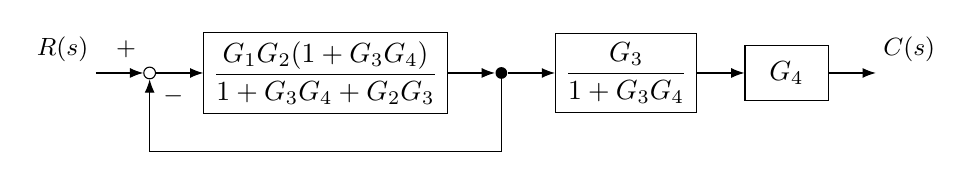
\begin{tikzpicture}[auto, node distance=0.4cm and 0.6cm, >=Latex]

  % 主系列ノード配置
  \node at (0,0) (input) {};
  \node[circle, draw, inner sep=1.5pt, right=of input] (sum1) {};
  \node[block, right=of sum1] (G1G2fb) 
    {$\dfrac{G_1 G_2 (1 + G_3 G_4)}{1 + G_3 G_4 + G_2 G_3}$}; % ← G1をかけた形
  \node[circle, fill=black, inner sep=1.5pt, right=of G1G2fb] (branch1) {};
  \node[block, right=of branch1] (G3_fb) {$\dfrac{G_3}{1 + G_3 G_4}$};
  \node[block, right=of G3_fb] (G4_main) {$G_4$};
  \node[right=of G4_main] (output) {};

  % 経由ポイント(sum1フィードバック用)
  \coordinate (pivot1) at ($(branch1)+(0,-1.0)$);

  % 主系列経路
  \draw[->] (input) -- (sum1);
  \draw[->] (sum1) -- (G1G2fb);
  \draw[->] (G1G2fb) -- (branch1);
  \draw[->] (branch1) -- (G3_fb);
  \draw[->] (G3_fb) -- (G4_main);
  \draw[->] (G4_main) -- (output);

  % フィードバック経路
  \draw[->] (branch1) -- (pivot1) -| (sum1);

  % 加算記号
  \node at ($(sum1)+(-0.3,0.3)$) {\small $+$};
  \node at ($(sum1)+(0.3,-0.3)$) {\small $-$};

  % ラベル
  \node at ($(input)+(-0.3,0.3)$) {\small $R(s)$};
  \node at ($(output)+(0.3,0.3)$) {\small $C(s)$};

\end{tikzpicture}



\vspace{2mm}
    
\begin{tikzpicture}
    \node {\Huge$\Downarrow$};
    \end{tikzpicture}
\vspace{2mm}

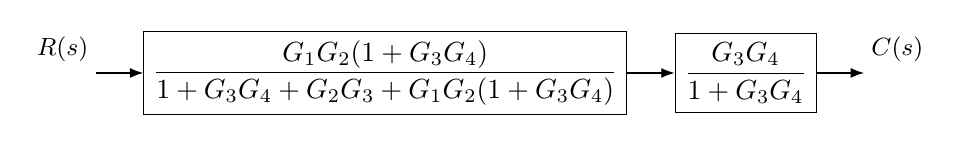
\begin{tikzpicture}[auto, node distance=0.4cm and 0.6cm, >=Latex]

  % ノード配置
  \node at (0,0) (input) {};
  \node[block, right=of input] (Gleft) 
    {$\dfrac{G_1 G_2 (1 + G_3 G_4)}{1 + G_3 G_4 + G_2 G_3 + G_1 G_2 (1 + G_3 G_4)}$};
  \node[block, right=of Gleft] (Gright) 
    {$\dfrac{G_3 G_4}{1 + G_3 G_4}$};
  \node[right=of Gright] (output) {};

  % 矢印
  \draw[->] (input) -- (Gleft);
  \draw[->] (Gleft) -- (Gright);
  \draw[->] (Gright) -- (output);

  % ラベル
  \node at ($(input)+(-0.3,0.3)$) {\small $R(s)$};
  \node at ($(output)+(0.3,0.3)$) {\small $C(s)$};

\end{tikzpicture}


\vspace{2mm}
    
\begin{tikzpicture}
    \node {\Huge$\Downarrow$};
    \end{tikzpicture}
\vspace{2mm}

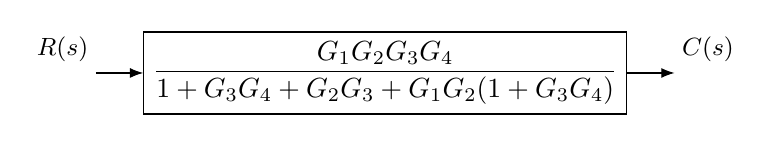
\begin{tikzpicture}[auto, node distance=0.4cm and 0.6cm, >=Latex]

  % ノード配置
  \node at (0,0) (input) {};
  \node[block, right=of input] (Gfinal) 
    {
    $\dfrac{
      G_1 G_2 G_3 G_4
    }{
      1 + G_3 G_4 + G_2 G_3 + G_1 G_2 (1 + G_3 G_4)
    }$
    };
  \node[right=of Gfinal] (output) {};

  % 矢印
  \draw[->] (input) -- (Gfinal);
  \draw[->] (Gfinal) -- (output);

  % ラベル
  \node at ($(input)+(-0.3,0.3)$) {\small $R(s)$};
  \node at ($(output)+(0.3,0.3)$) {\small $C(s)$};

\end{tikzpicture}


\end{center}

\end{tcolorbox}

\end{document}